\section{Results}
\label{sec:results}
\subsection{Energy management without malicious participants}
In the clean 500-day experiments with validation-selected policies, FedAvg curtails approximately 145\,kWh per household annually, compared with 473\,kWh under the self-consumption rule, a reduction of about 69\%. FedProx and local SAC also reduce curtailment. Across these three learning methods, street-wide charging during designated MSL intervals is approximately 12,400--13,300\,kWh, compared with 1,971\,kWh for the rule. Figure~\ref{fig:energy} and Table~\ref{tab:clean_energy} distinguish these energy outcomes from electricity bills.

Bill differences from the rule are smaller. The rule costs approximately \$953 per household annually; FedAvg, FedProx and local SAC average \$954, \$947 and \$964, respectively, with wide three-seed intervals. Central SAC averages \$879 and perfect-foresight MPC \$591. These references use additional information: central SAC pools household data, and MPC receives exact daily future profiles. The clean results therefore show lower curtailment more clearly than a bill advantage of federation over the rule.

The reduction in curtailment is accompanied by greater battery throughput. FedAvg produces approximately 256 fleet-equivalent cycles annually, compared with 77 for the rule. Because the objective does not monetise this cycling, electricity bills alone do not establish net economic value after degradation and capital costs. These clean outcomes provide the operational context for the attack comparisons. Table~\ref{tab:extended_clean} reports all 1000-day and FedProx-coefficient runs. Mean bills at 1000 days are approximately \$902 for FedAvg, \$890 for FedProx, \$927 for local SAC and \$810 for central SAC; these duration comparisons use validation-selected actors and do not alter the 500-day attack protocol.

\begin{figure}[htbp]
\centering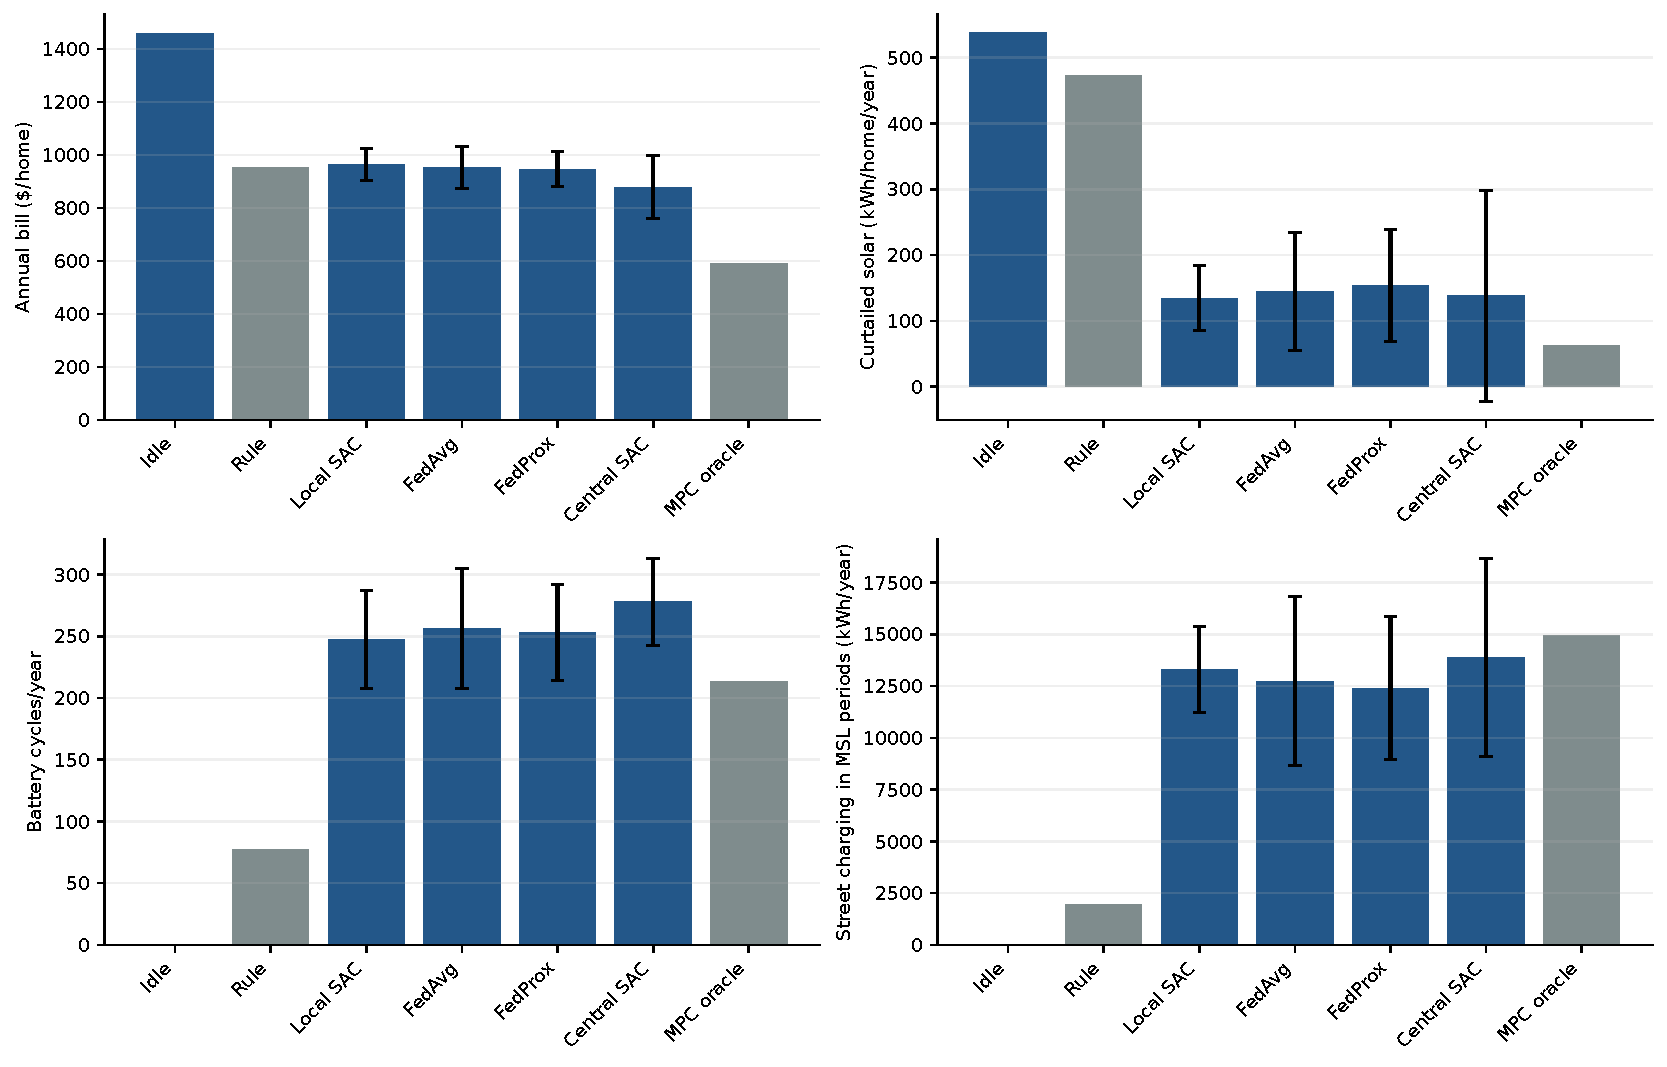
\includegraphics[width=\linewidth]{figures/clean_energy.pdf}
\caption{Clean 500-day energy-management outcomes on Ausgrid. Error bars show Student-$t$ 95\% interval half-widths over three learning seeds. Deterministic baselines have no seed interval. MSL charging is a street total; bill and curtailment are household averages, and cycling is fleet-equivalent. MPC uses perfect daily foresight.}
\label{fig:energy}
\end{figure}

\subsection{Damage under compromised learning contributions}
Table~\ref{tab:ausgrid_damage} reports five-seed Ausgrid damage under all six attacks. FedAvg has mean annual damage of approximately \$532 per household under noise and \$527 under Normalized. Coordinate median and trimmed mean limit some perturbations but retain Normalized damage of approximately \$254 and \$248. Thus, suppressing extreme coordinates does not remove the observed vulnerability to directional poisoning.

Final FedGrid has mean Normalized damage of approximately \$11, compared with \$88 for the original method. Its largest attack-wise mean is approximately \$64 under flip, followed by \$63 under reward poisoning. For comparison, the largest attack-wise means are approximately \$23 for FLTrust, \$50 for FLAME and \$38 for tuned TAFDRL-style. These are descriptive maxima across attacks; the wide seed intervals do not establish a statistical ranking or uniform superiority of final FedGrid.

The final configuration's Normalized estimate has an interval half-width of approximately \$59. Its low mean consequently does not establish immunity, and the comparison remains conditional on the reference data, finite attack search and fixed household assignment.
\begin{table}[ht]
\centering\scriptsize
\caption{Ausgrid annual bill damage, seeds 0--4. Entries are mean $\pm$ 95\% confidence interval half-width [seeds], in dollars per household. These are intervals for each attack, not for the maximum across attacks.}
\label{tab:ausgrid_damage}
\resizebox{\linewidth}{!}{%
\begin{tabular}{lrrrrrr}
\toprule
Method & Flip & Scale & Noise & Normalized & Meter & Reward \\
\midrule
FedAvg & 100 $\pm$ 70 [5] & 36 $\pm$ 74 [5] & 532 $\pm$ 92 [5] & 527 $\pm$ 78 [5] & -3 $\pm$ 42 [5] & 42 $\pm$ 46 [5] \\
median & 78 $\pm$ 70 [5] & -8 $\pm$ 28 [5] & -12 $\pm$ 27 [5] & 254 $\pm$ 132 [5] & -10 $\pm$ 11 [5] & 79 $\pm$ 48 [5] \\
trimmed & 64 $\pm$ 27 [5] & -18 $\pm$ 16 [5] & -7 $\pm$ 25 [5] & 248 $\pm$ 77 [5] & -8 $\pm$ 13 [5] & 83 $\pm$ 26 [5] \\
Krum & 41 $\pm$ 99 [5] & 35 $\pm$ 72 [5] & 3 $\pm$ 51 [5] & 47 $\pm$ 98 [5] & 27 $\pm$ 42 [5] & 44 $\pm$ 88 [5] \\
FLTrust & -4 $\pm$ 18 [5] & 4 $\pm$ 4 [5] & -14 $\pm$ 33 [5] & 23 $\pm$ 67 [5] & 19 $\pm$ 6 [5] & 20 $\pm$ 37 [5] \\
FLAME & 50 $\pm$ 58 [5] & 10 $\pm$ 40 [5] & 2 $\pm$ 28 [5] & 43 $\pm$ 55 [5] & 10 $\pm$ 40 [5] & -2 $\pm$ 41 [5] \\
TAFDRL-style & 89 $\pm$ 44 [5] & 14 $\pm$ 16 [5] & -6 $\pm$ 43 [5] & 66 $\pm$ 86 [5] & 15 $\pm$ 22 [5] & 6 $\pm$ 31 [5] \\
TAFDRL-style final & 34 $\pm$ 8 [5] & 21 $\pm$ 25 [5] & -4 $\pm$ 33 [5] & 38 $\pm$ 107 [5] & 6 $\pm$ 26 [5] & 20 $\pm$ 39 [5] \\
FedGrid & 74 $\pm$ 51 [5] & -4 $\pm$ 13 [5] & 47 $\pm$ 24 [5] & 88 $\pm$ 11 [5] & 12 $\pm$ 37 [5] & 48 $\pm$ 53 [5] \\
FedGrid final & 64 $\pm$ 47 [5] & -9 $\pm$ 17 [5] & 19 $\pm$ 34 [5] & 11 $\pm$ 59 [5] & 25 $\pm$ 33 [5] & 63 $\pm$ 56 [5] \\
\bottomrule
\end{tabular}}
\end{table}

\begin{figure}[htbp]
\centering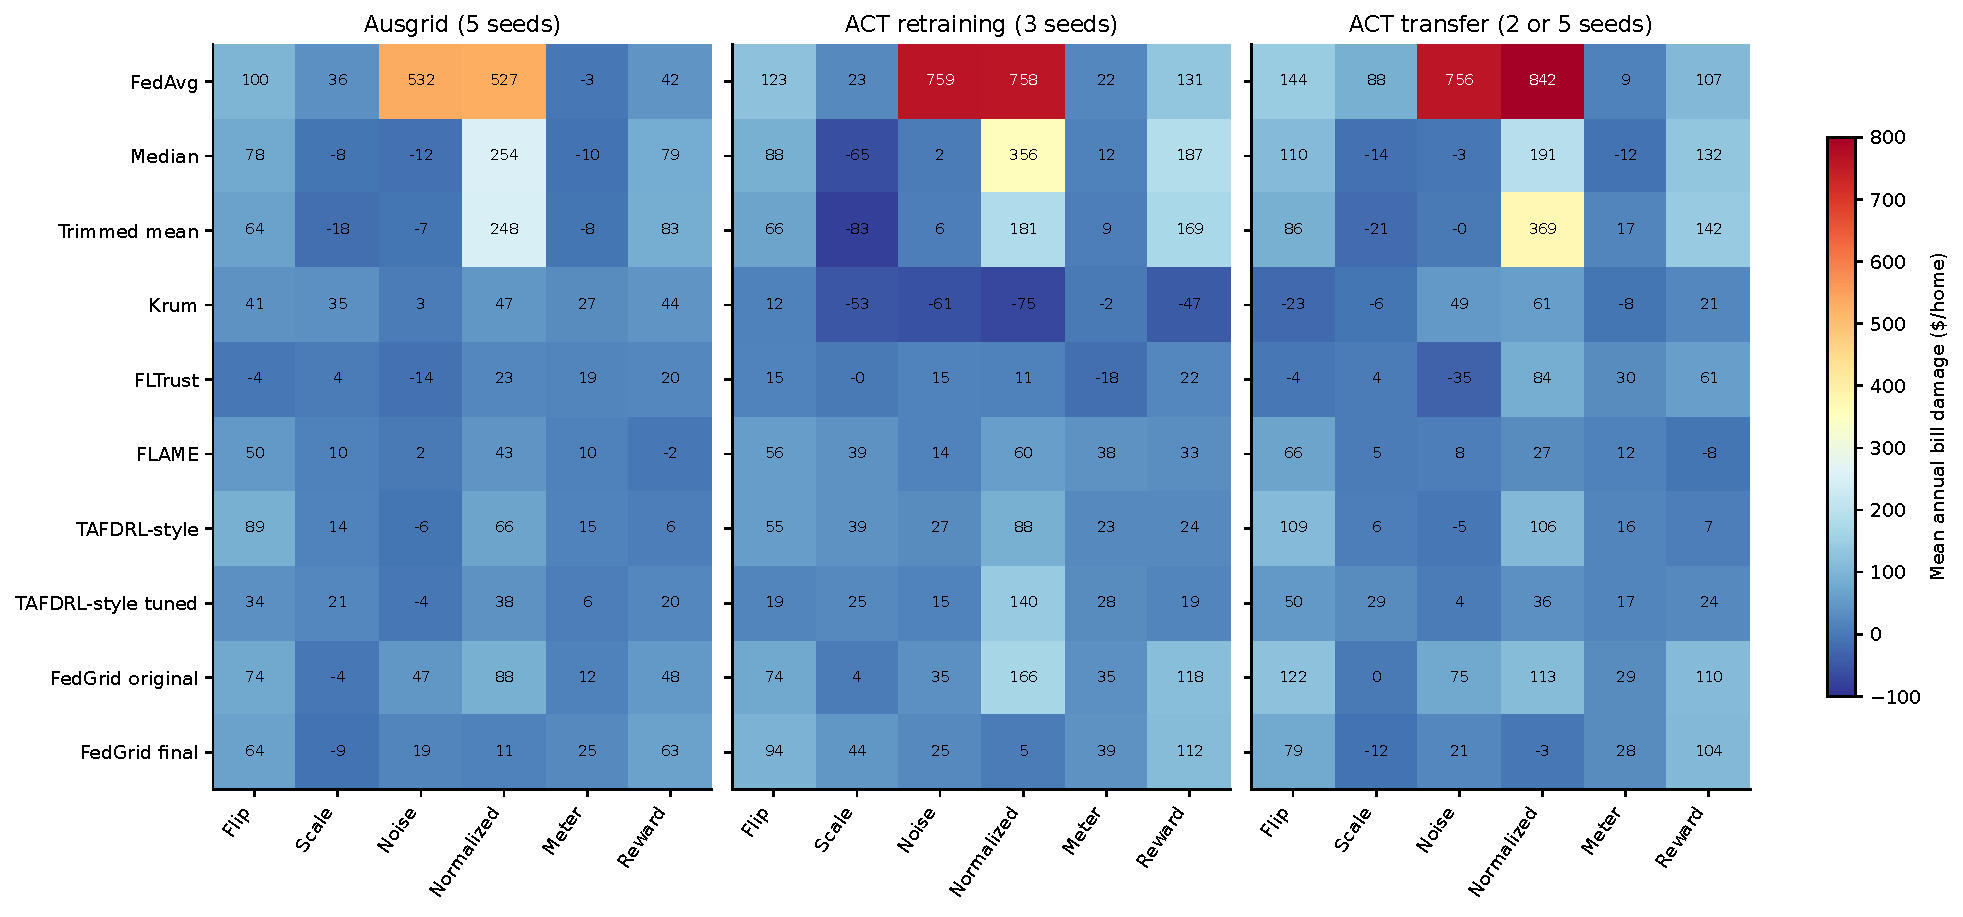
\includegraphics[width=\linewidth]{figures/attack_damage.pdf}
\caption{Mean annual bill damage across six attacks. The same colour scale is used for Ausgrid, ACT retraining and ACT transfer. Transfer uses two seeds for original methods and five for final variants; these unequal means are not paired revision estimates. Update attacks evaluate all homes, while meter and reward attacks evaluate matched honest homes.}
\label{fig:damage}
\end{figure}

\subsection{ACT retraining and transfer}
In three-seed ACT retraining, mean Normalized damage falls from approximately \$166 for original FedGrid to \$5 for the final configuration. Final FedGrid nevertheless incurs approximately \$112 under reward poisoning and \$94 under flip. Table~\ref{tab:act_damage} shows that the attack profile changes with the household data even when feeder and tariff assumptions are retained. These outcomes remain subject to the ACT imputation overlap.


Transfer applies the Ausgrid-trained shared policy and local output layers to ACT households at the corresponding feeder positions without retraining. Final FedGrid has five available seeds; original FedGrid and most comparators have two. The final configuration's five-seed mean Normalized damage is approximately $-\$3$, with an interval half-width of \$60. Reward damage is approximately \$104, with a half-width of \$40, indicating persistent sensitivity to training-time reward corruption. Differences between these unequal method means are not matched revision effects.

\subsection{Matched effect of the FedGrid revision}
Table~\ref{tab:paired_revision} and Figure~\ref{fig:paired} compare final and original FedGrid using matched seeds and attacks. The paired Normalized change in annual damage is $-\$76.8\pm\$67.5$ on Ausgrid and $-\$160.6\pm\$97.5$ on ACT. The descriptive Student-$t$ intervals exclude zero, but the five-pair Ausgrid exact test gives $p=0.0625$ and $p_{\mathrm{Holm}}=0.375$ within the six-attack revision family. We report the estimated reduction without a multiplicity-controlled improvement claim. Transfer gives $-\$74.1\pm\$175.9$ on the two common seeds, demonstrating the limited precision of the matched estimate.

The revision does not lower every observed attack mean. ACT scale damage changes by approximately +\$40, and Ausgrid meter damage by approximately +\$14. Their broad intervals do not establish systematic deterioration; they nevertheless qualify an interpretation based only on the favourable Normalized result.

\begin{figure}[htbp]
\centering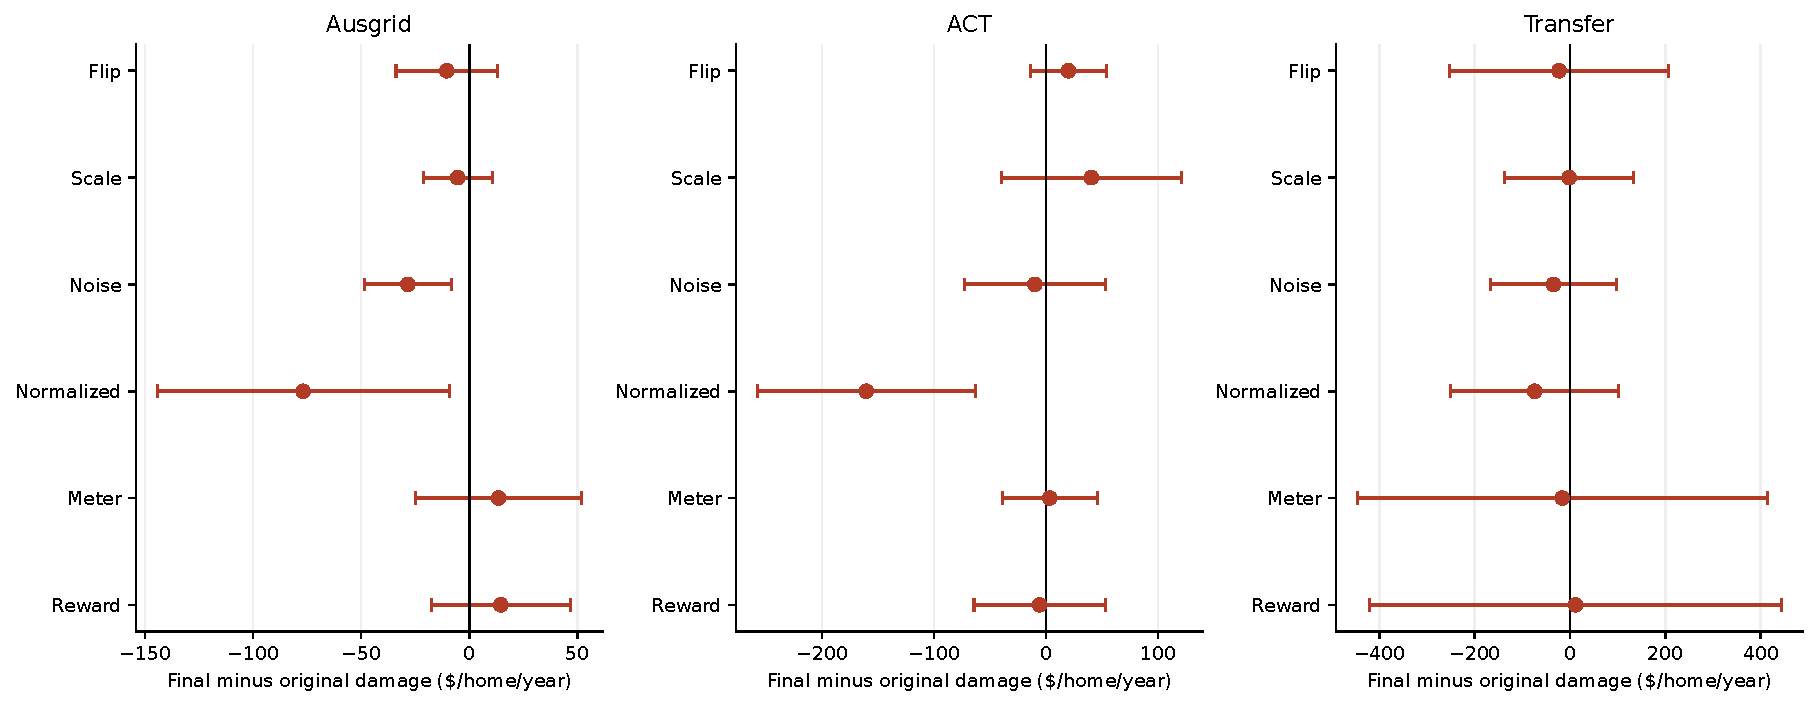
\includegraphics[width=\linewidth]{figures/paired_revision.pdf}
\caption{Matched final-minus-original change in annual attack damage. Negative values favour the revision. Error bars are unadjusted 95\% Student-$t$ intervals over five Ausgrid, three ACT or two common transfer seeds. The horizontal scales vary to display the substantially greater transfer uncertainty.}
\label{fig:paired}
\end{figure}

\subsection{Recorded rejection and the apparent trade-off}
Figure~\ref{fig:tradeoff} plots the largest attack-wise mean bill damage against mean logged honest rejection, with matching seed scopes within each panel. Final FedGrid records fewer rejected honest vectors than several comparators and lower noise and Normalized damage than FedAvg. FedAvg, median and trimmed mean are omitted from the scatter because their logs provide no comparable whole-vector rejection rate.

The horizontal coordinate has method-specific admission semantics and omits zero-weight FedGrid groups. The scatter therefore describes logged behaviour rather than a common participation frontier. Lower rejection does not establish that more households contribute positive weight, and the same qualification applies to the post-hoc eligibility bound.

Table~\ref{tab:rejection} and Figure~\ref{fig:rejection} retain attack-specific rates, observation counts and no-attack references. Krum's high rate reflects its single-vector selection rule. Some older Krum logs lack rejection statistics; summaries use the available observations without reconstructing missing histories.
\begin{figure}[htbp]
\centering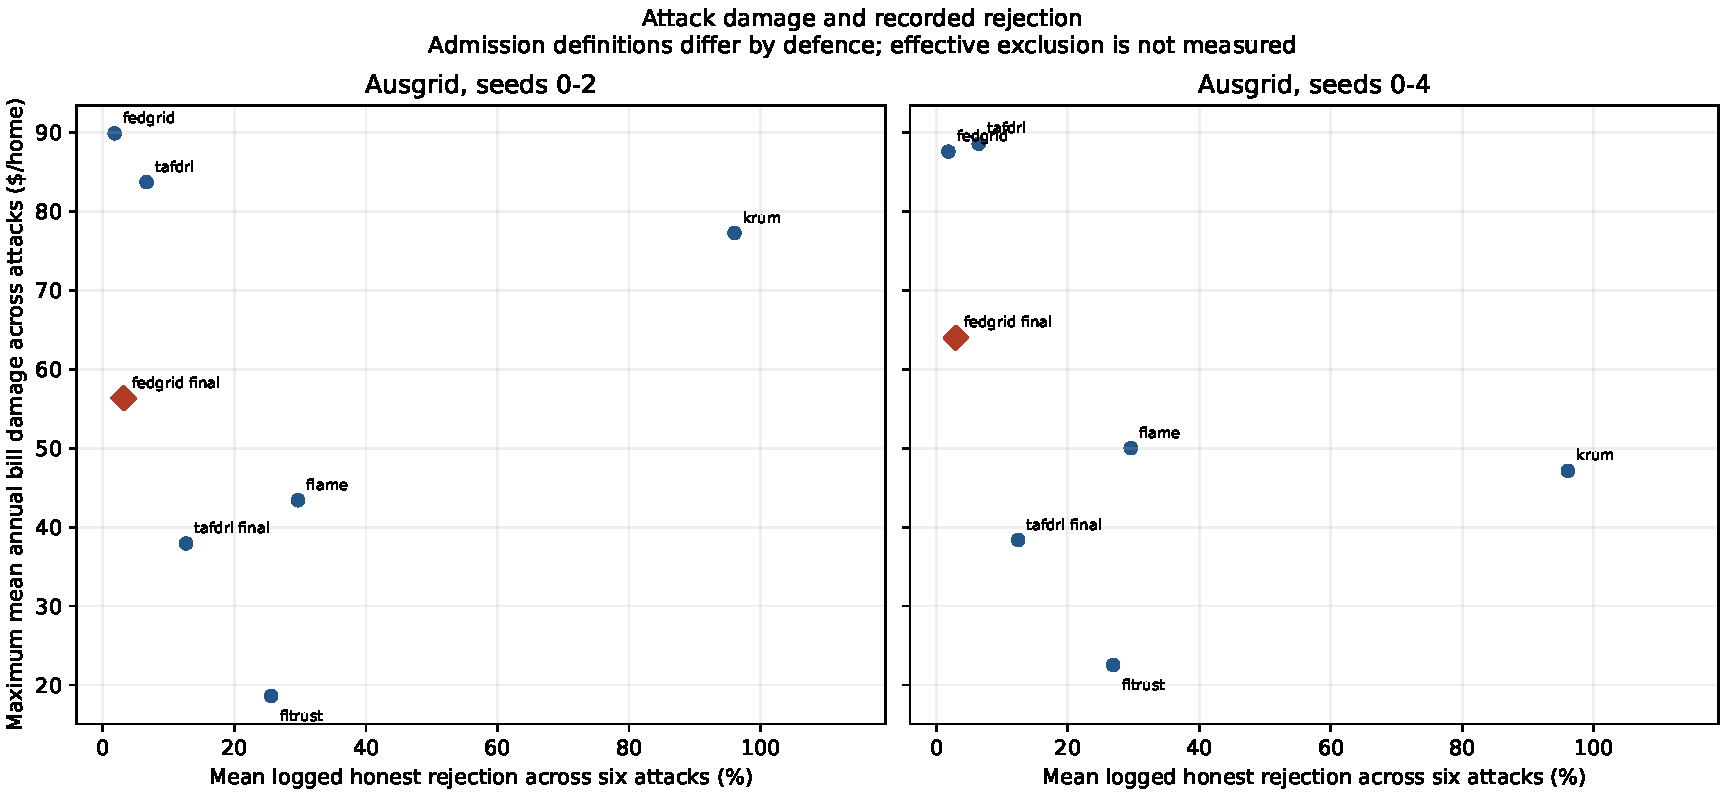
\includegraphics[width=\linewidth]{figures/damage_rejection.pdf}
\caption{Worst-case mean annual bill damage against mean logged honest rejection over the six attacks, at nominal 30\% compromise. Panels use seeds 0--2 and 0--4. Rejection definitions differ across methods and omit zero-weight groups for FedGrid. The vertical coordinate is the maximum of attack means, without an asserted confidence interval for that maximum.}
\label{fig:tradeoff}
\end{figure}

\begin{figure}[htbp]
\centering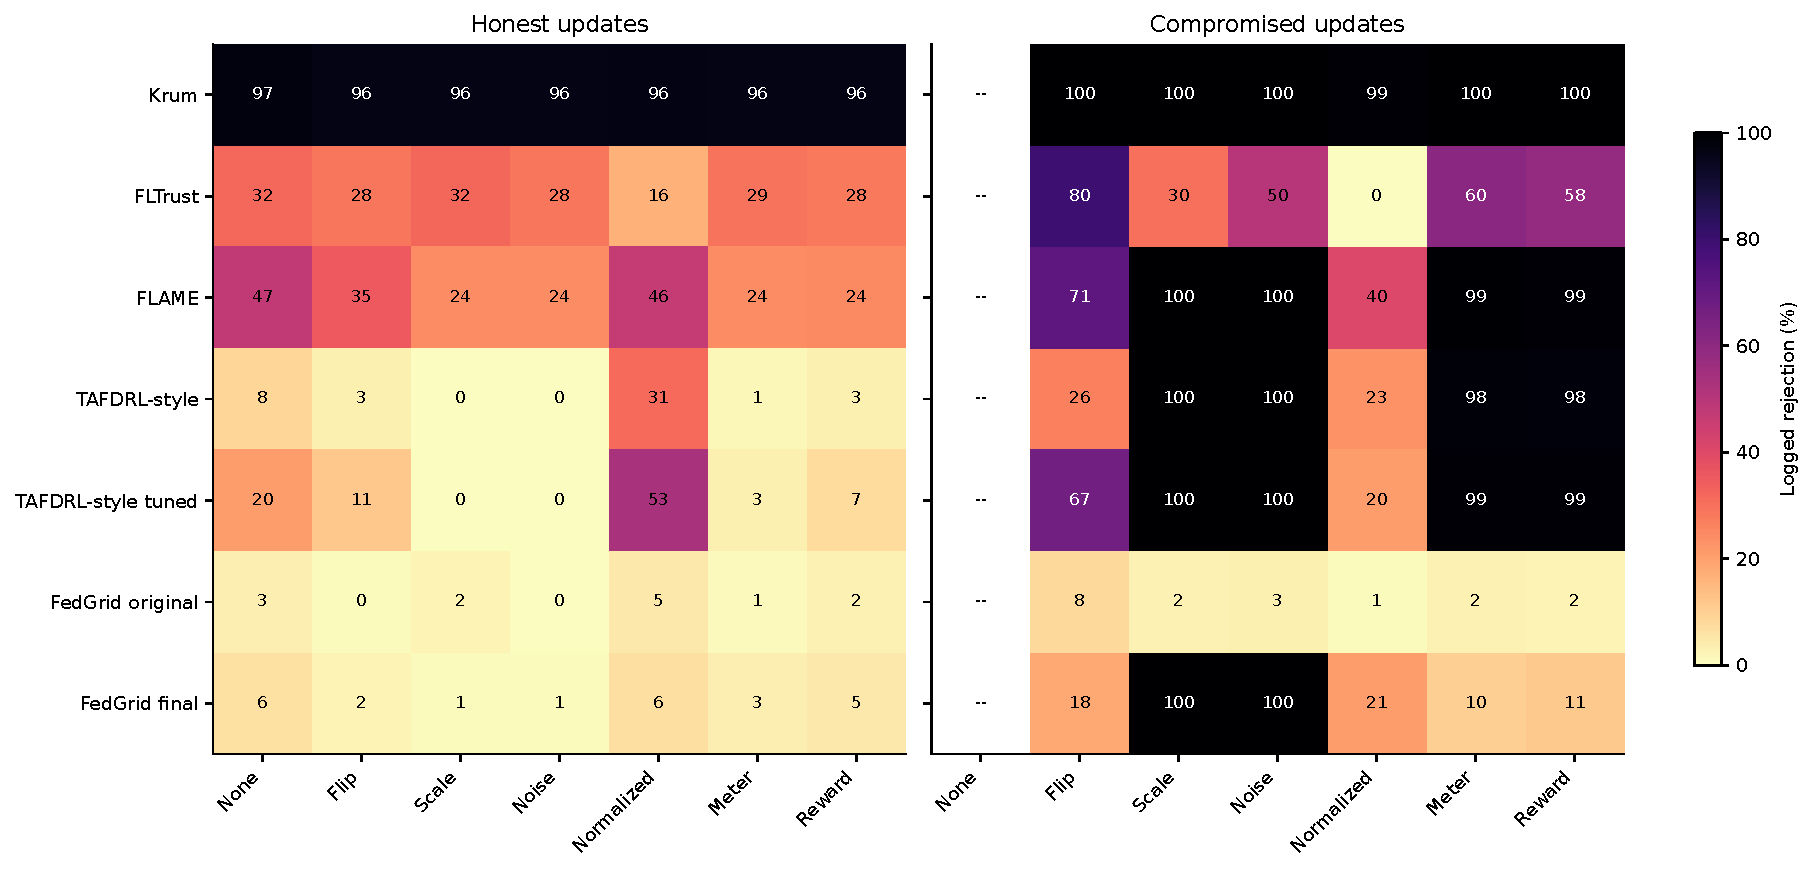
\includegraphics[width=\linewidth]{figures/rejection_heatmap.pdf}
\caption{Mean logged rejection of honest and compromised updates on Ausgrid, seeds 0--4 where available. Dashes indicate unavailable statistics, including compromised rejection in no-attack runs. The values describe method-specific admission decisions, not a uniformly defined exclusion event.}
\label{fig:rejection}
\end{figure}

\subsection{Electrical outcomes and observed violations}
Table~\ref{tab:electrical} reports voltage and transformer outcomes for the no-attack last-policy references, and Figure~\ref{fig:electrical} compares transformer peaks. Each run contributes its peak over the evaluated intervals; the displayed mean and interval summarise those run-level peaks. They do not bound loading in other conditions. These electrical outcomes complement bill damage because simultaneous charging can alter feeder loading even when household costs remain low.



Small voltage-exceedance rates are present in the no-attack logs and are retained at three-decimal precision in Table~\ref{tab:electrical}. Final FedGrid's five-seed mean is $0.010\pm0.028\%$, calculated from the logged rounded rates; its seed-4 run records 0.05\% exceedance and a maximum of 253.60\,V. Averaging run maxima does not make that individual violation disappear.

Attack-time physical outcomes also matter. Table~\ref{tab:attack_electrical} reports maxima over every principal attack run. Under Normalized poisoning, FedAvg reaches transformer peaks of 108.89\% and 113.84\% in seeds 1 and 4. In the single-seed 1.02\,pu final FedGrid no-attack case, the recorded voltage-exceedance rate is 0.27\% and maximum voltage is 254.09\,V. These observations demonstrate why enforced export allowances must be distinguished from voltage and transformer guarantees.
